\documentclass[tikz]{standalone}
% \usepackage{tikz} % already loaded by the documentclass
\usepackage{braket}
\usetikzlibrary{arrows.meta}
\begin{document}
%%| filename: bloch-sphere
%%| header-includes: \usetikzlibrary{arrows.meta}
%%| additionalPackages: \usepackage{braket}
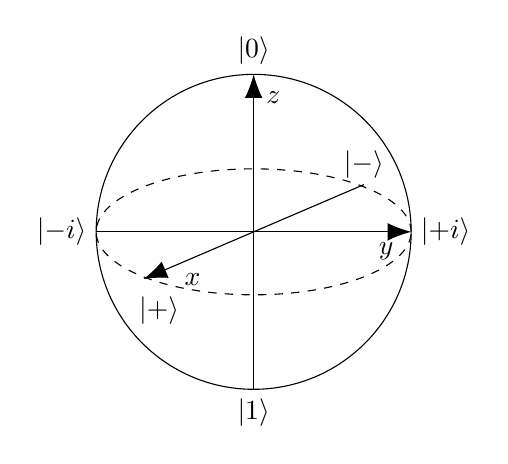
\begin{tikzpicture}[scale=2]
    % Draw main circle
    \draw (0,0) circle (1);
    
    % Draw ellipse for perspective
    \draw[dashed] (0,0) ellipse (1 and 0.4);
    
    % Draw axes
    \draw[-{Latex[length=3mm]}] (-1.0,0) -- (1.0,0) node[below=2.5mm,left=1mm] {$y$};
    \draw[-{Latex[length=3mm]}] (0,-1.0) -- (0,1.0) node[right=2.5mm,below=1mm] {$z$};
    \draw[-{Latex[length=3mm]}] (0.7,0.3) -- (-0.7,-0.3) node[right=4mm] {$x$};
    
    % Label states
    % Z basis
    \node[above] at (0,1) {$\ket{0}$};
    \node[below] at (0,-1) {$\ket{1}$};
    
    % Y basis
    \node[right] at (1,0) {$\ket{+i}$};
    \node[left] at (-1,0) {$\ket{-i}$};
    
    % X basis
    \node[right=2mm, above=0.5mm] at (0.6,0.25) {$\ket{-}$};
    \node[below=2mm] at (-0.6,-0.25) {$\ket{+}$};
\end{tikzpicture}
\end{document}
      